\newpage
\section{Giới thiệu chung}
\subsection{Giới thiệu chung về OpenMP}
Lập trình đa luồng là một phương pháp lập trình trong đó một chương trình có khả năng thực hiện nhiều công việc đồng thời, mỗi công việc được thực hiện trong một luồng riêng biệt.

OpenMP (Open Multi-Processing) là một giao diện lập trình ứng dụng   hỗ trợ lập trình đa xử lý bộ nhớ dùng chung đa nền tảng trong C , C++ và Fortran.

OpenMP được thiết kế cho các máy đa bộ xử lý, bộ nhớ dùng chung. Kiến trúc cơ bản có thể là bộ nhớ chia sẻ UMA hoặc NUMA.           Chia sẻ bộ nhớ     trong đó nhiều luồng có thể truy cập cùng một không gian bộ nhớ chung.  

\begin{figure}[h]         
    \centering
    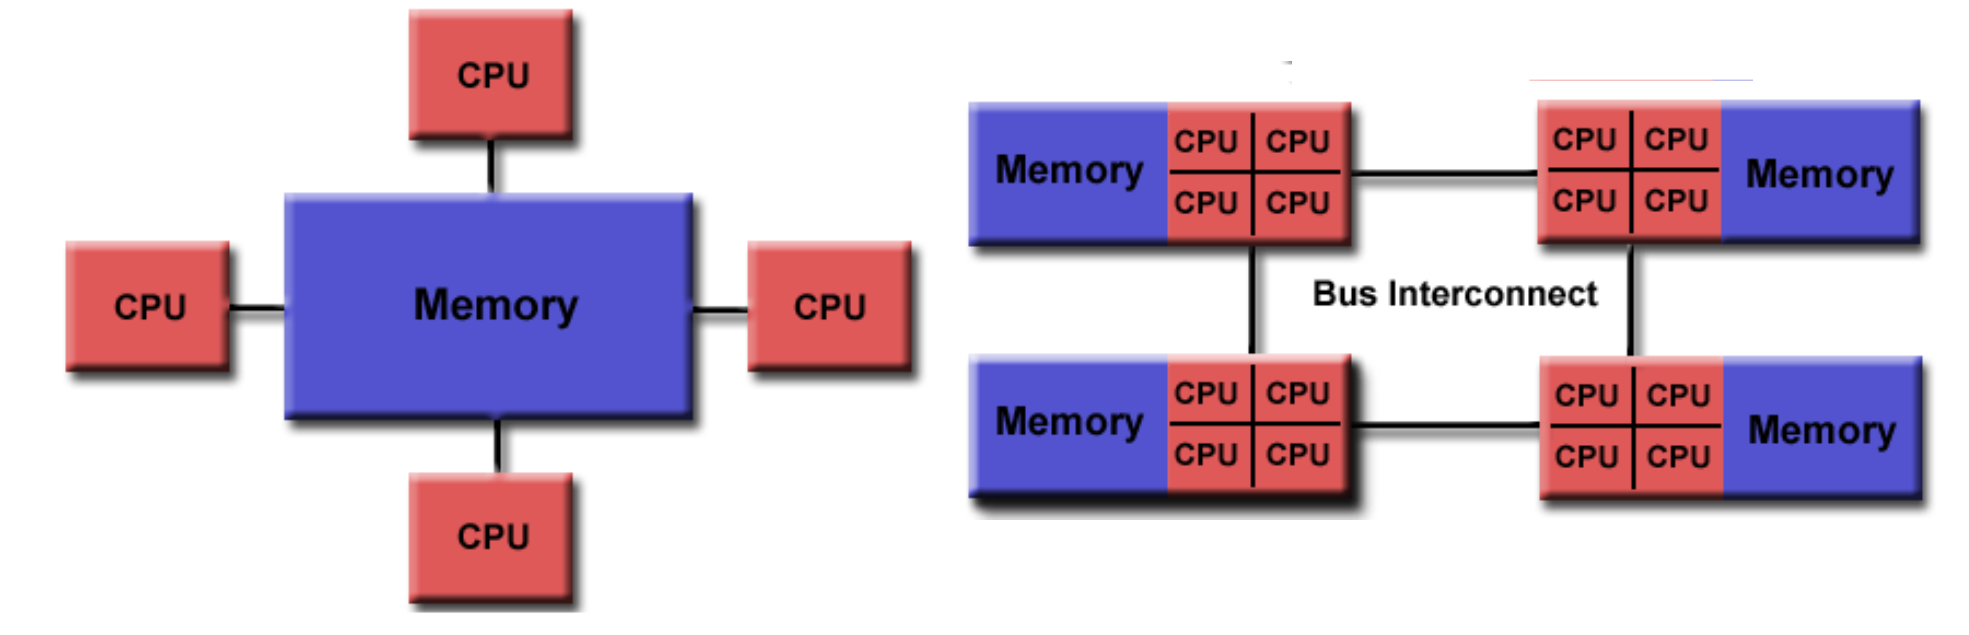
\includegraphics[width=1\textwidth]{pictures/000.png}         
    \caption{ViDuHinhAnhTheoChieuNgang}         
    \label{pictures:000}         
    \end{figure} 
    
    
    
OpenMP sử dụng mô hình fork-join để thực thi song song:
 
\begin{figure}[h]         
    \centering
    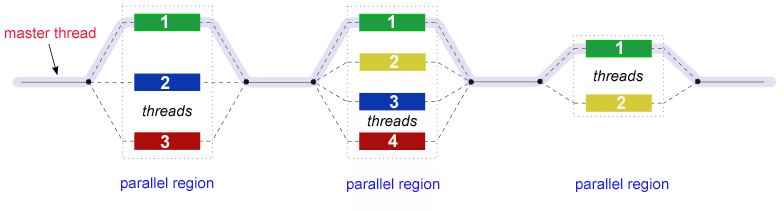
\includegraphics[width=1\textwidth]{pictures/Fork-Join-model-WebSite-4.png}         
    \caption{ViDuHinhAnhTheoChieuNgang}         
    \label{pictures:0001}         
    \end{figure} 



Tất cả các chương trình OpenMP đều bắt đầu dưới dạng một tiến trình duy nhất: luồng chính . Luồng chính thực thi tuần tự cho đến khi gặp cấu trúc vùng song song đầu tiên.


 
\textbf{FORK:}   luồng chính sau đó tạo ra một nhóm các luồng song song .

Sau đó, các câu lệnh trong chương trình được bao quanh bởi cấu trúc vùng song song sẽ được thực thi song song giữa các luồng nhóm khác nhau.

\textbf{JOIN:}         Khi các luồng của nhóm hoàn thành các câu lệnh trong cấu trúc vùng song song, chúng sẽ đồng bộ hóa và chấm dứt, chỉ để lại luồng chính.

 
 
 
 
\newpage
\subsection{Công thức tính hiệu suất}


Công thức tính hiệu suất trong bài báo cáo: 
 

\[\text{{Hiệu suất}} = \frac{{\text{{Thời gian tuần tự}}}}{{\text{{Thời gian song song}} \times \text{{Số luồng}}}}\]
 
 
\subsection{Thông tin về máy tính và phần mềm}


\begin{table}[h]
    \centering
    \begin{tabular}{|l|l|}
        \hline
        \textbf{Thông Tin CPU} & Intel(R) Core(TM) i5-9300H CPU @ 2.40GHz \\
        \hline
        \textbf{Thông Tin RAM} & 16.0 GB \\
        \hline
        \textbf{Hệ Điều Hành} & Windows 11 \\
        \hline
        \textbf{Ngôn Ngữ Lập Trình} & C, C++ \\
        \hline
        \textbf{Trình Biên Dịch} & g++ \\
        \hline
    \end{tabular}
    \caption{Thông Tin Hệ Thống}
    \label{table:system-info}
\end{table}